\section{System Overview}

% Overview
Our 3DTI system fuses two distributed scenes into a virtual space in full 3D. The end-to-end delay is 50 ms, i.e., the time interval between a user acts and his remote partner sees. The system consists of inexpensive commercial devices (\$ 7000). Figure xxx illustrates the pipeline of our system. In particular, the system removes background and retained only individuals and similar objects in both scenes.

The project is open-source [?]. The motivation of this section is to provide necessary information for the readers to rebuild a similar system.

%Each side: CPU $400; GPU $700; network card $400; RAM $200; Disk $200; HTC Vive $1200; Realsense $150*3.

\subsection{Hardware and Software Overview}

\subsubsection{Hardware}

The system consists of two capture sites in the two distributed rooms. At each capture site, we had three depth cameras for capturing, a PC for computing and an HMD for rendering. Realsense D415 (depth cameras) were used to capture a volume of $2m \times 2m \times 2m$. The locating place of each camera and its contribution to 3D mesh are illustrated in Figure xx. Each PC had an Intel i7-7700k CPU and a GTX 1080Ti GPU. HTC Vive was used to present the fused reconstruction of both sides. Ten Gigabit network cards (Intel X520-SR2) were used to connect the two capture sites.

\subsubsection{Software}

OpenCV was used for camera calibration. CUDA was used for image processing and the kernel algorithm. Unity3D was used to implement the high-level application. It fetches live reconstruction from the kernel and renders it in HTC Vive. Python was used for audio transmission.

\subsection{Calibration}

\subsubsection{Calibration between Cameras}

The \emph{camera calibration module} in OpenCV was used to calibrate the cameras. Each pair of cameras took ten snapshots (1080p color images) of a glass-made flat checkerboard. Then, OpenCV aligned their coordinates ($SD < 1 pixel$).

\subsubsection{Calibration between HMD and Cameras}

The HTC Vive was calibrated by setting the original point in its software. We placed the original point of the cameras at the same position by using the checkerboard. Hence, we aligned the HTC Vive with the cameras. This calibration is not necessarily accurate because the users can hardly perceive the error [?]. This step also aligned the coordinates of the two capture sites.

\subsection{Preprocessing}

\subsubsection{Depth Processing}

The cameras acquired depth images of $640 \times 480$ pixels at 30 FPS. The Realsense D415 is based on binocular disparity. Thus, disparity values (instead of depth values) were used in the processing to improve accuracy. We applied median filtering, spatial filtering, hole filling and temporary filtering on the depth images.

\subsubsection{Color Processing}

The cameras acquired color images of $960 \times 540$ pixels at 30 FPS. The exposure settings were manually adjusted. We used one RGB camera as a reference and warped the other cameras to this reference by white balancing and linear mapping.

\subsubsection{Background Removal}

The system removed unnecessary background and retained only shared objects and individuals. In the calibration step, we recorded RGBD images as the background. At runtime, we removed pixels that are similar to the background based on thresholds.

\subsection{3D Reconstruction}

3D reconstruction is the kernel algorithm of a 3DTI system. We developed a real-time CUDA implementation of 3D reconstruction similar to KinectFusion \cite{izadi2011kinectfusion}. First, the algorithm integrated depth images into a data structure named Truncated Signed Distance Function (TSDF) Volume \cite{curless1996volumetric}. Next, the 3D mesh was extracted from the TSDF Volume using Marching Cubes \cite{lorensen1987marching}. Then, the algorithm projected color images on the 3D mesh for colorization.

The resolution of TSDF volume was $256 \times 256 \times 256$ voxels. In the TSDF processing, we used a weighted average where $W = \frac{1}{Dist}$ on different cameras to minimize the error. In the colorization, we upsampled each triangle to four quartered parts to sample more colors (Figure \ref{fig:color_upsampling}). Because the users are more sensitive to the texture but not the shape [?].

\begin{figure}[H]
\centering
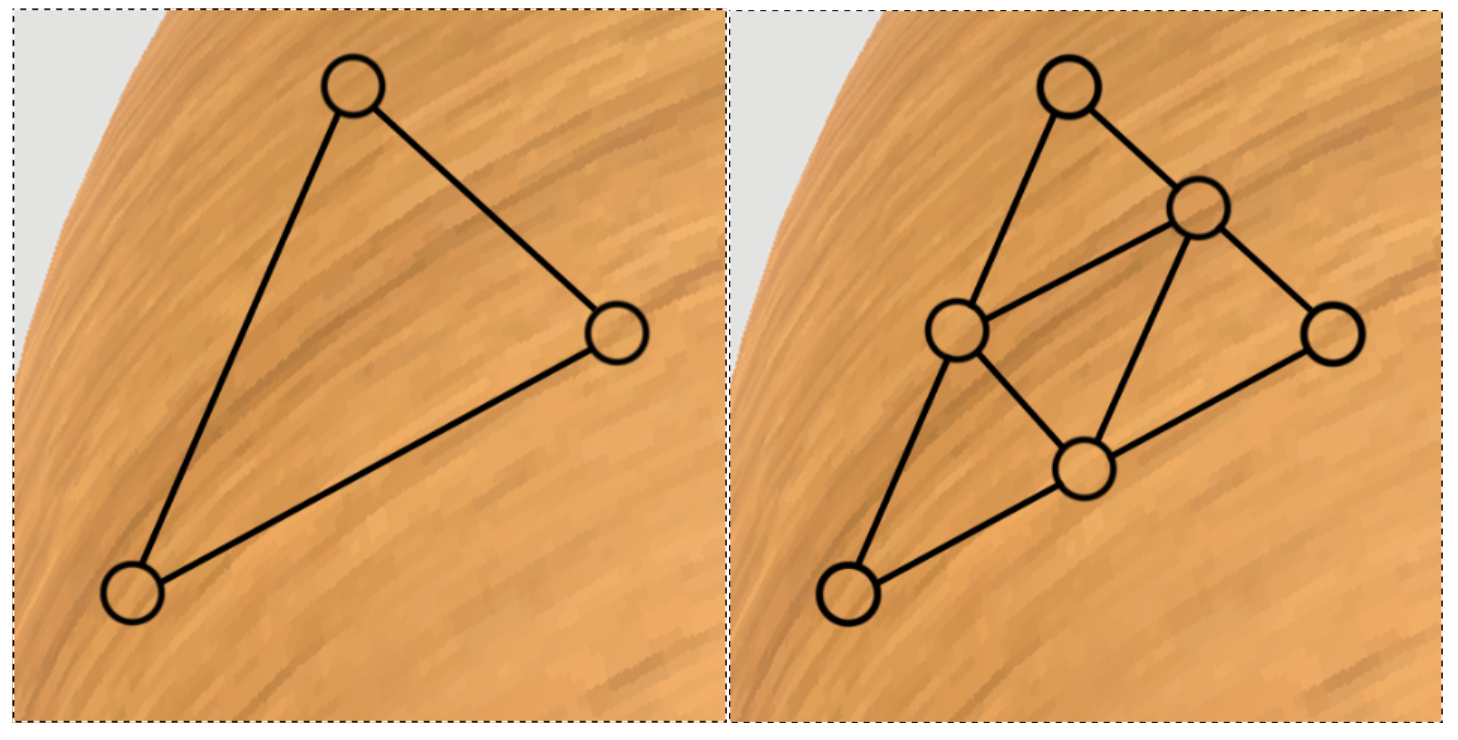
\includegraphics[width=0.8\linewidth]{figures/figure_mc.png}
\caption{Left: Mesh without Supersampling; Right: Mesh witht Supersampling.}
\label{fig:color_upsampling}
\end{figure}

我们修改了TSDF的方法,使得它能够融合两端的场景。
1、我觉得这段需要引入一些公式。
2、图做半版的就行了,还没到需要用长图的程度。
结合Figure \ref{fig:TSDF_merge_two_sides}来说。
    
%[from lwq] As we need to merge point clouds from two clients, we need to retain some objects from the other depth camera array. In one of our application, we fuse two chessboards along with half of the chess each side together to implement remote gaming. In this case, we need to retain the chess from both sides. So we run TSDF on each side separately and take the minimum of SDF values to gain the actual surface of the merged mesh. A simple example of this procession is shown in Figure XX.

[from lwq] We modify TSDF to adapt our demand of merging point clouds from two clients. Figure 3.4 is the weighted combination of the two profiles from different clients. The combination rules are:
\begin{equation}
V_z=\min\{\frac{\sum_{local} W_{i,z}S_{i,z}}{\sum_{local} W_{i,z}},\frac{\sum_{remote} W_{j,z}S_{j,z}}{\sum_{remote} W_{j,z}}\}
\end{equation}
\begin{equation}
W_{i,z}=\frac{1}{dist(i,z)}    
\end{equation}
where $S_{i,z}$ are SDF value of $z$th volume get by $i$th camera and $dist(i,z)$ is the distence from $i$th camera to $z$th volume. $V_z$ is the final SDF value of $z$th volume after combination.

\begin{figure}[!htbp]
\centering
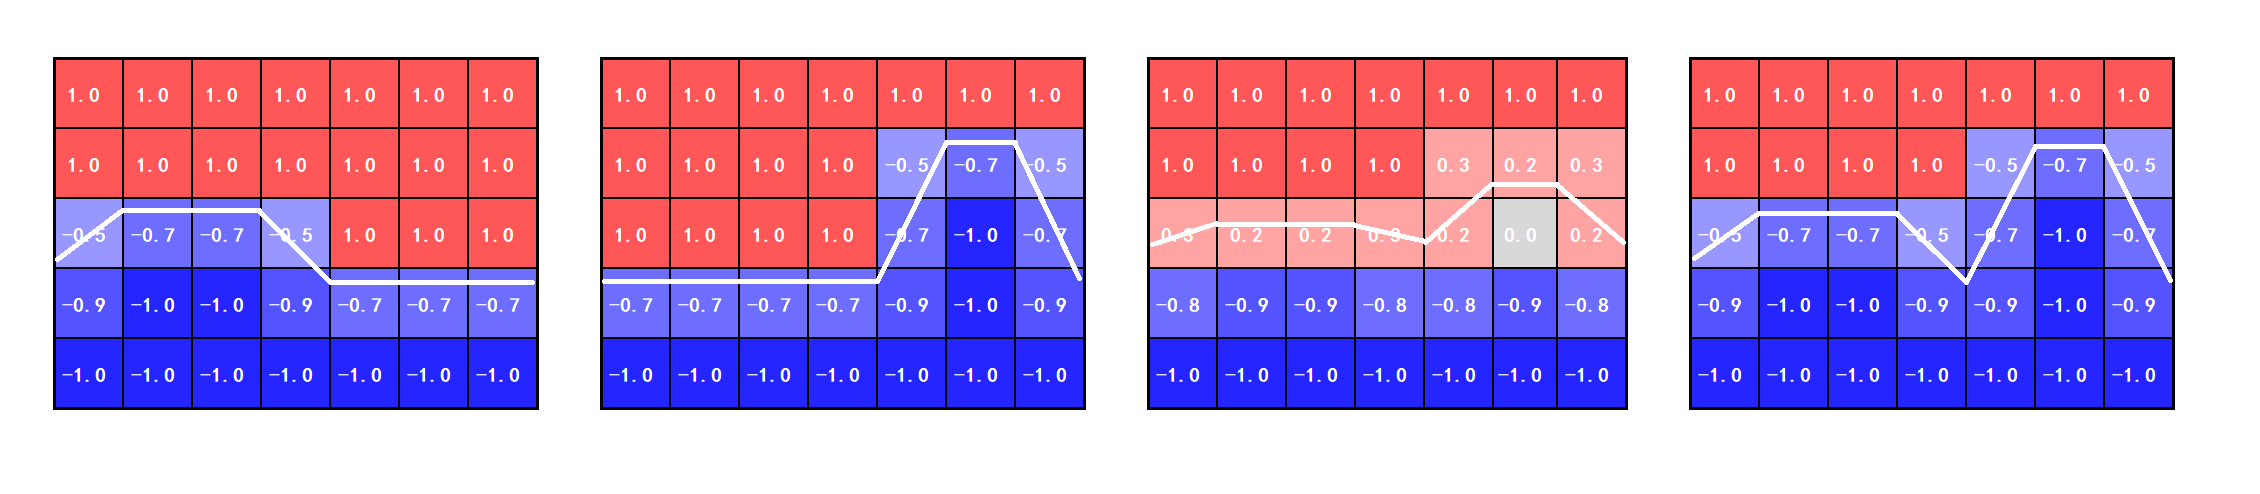
\includegraphics[width=1.0\linewidth]{figures/figure_tsdf.png}
\caption{Left to right: 1)SDF value from camera 1; 2)Merged SDF value from camera 2; 3)SDF value by simple average; 4)Merged SDF value from our project.}
\label{fig:TSDF_merge_two_sides}
\end{figure}

\subsection{End-to-end Delay}

The lowest end-to-end delay of our system was 52 ($\pm$ xx) ms. The frame rate of 3D reconstruction was 30 FPS. It was controlled by the frequency of the synchronized depth cameras. In average, a frame (33 ms) consisted of 19 ms processing and 14 ms idling. The remote images had one frame of latency. So the end-to-end delay was about $33 + 19 = 52$ ms. For artificial delay, we buffered remote data for frames. Figure \ref{fig:system_delay} shows the pipeline in details. Notice that the frame rate of rendering was 90 FPS so that the users did not feel dizzy.

\begin{figure}[!htbp]
\centering
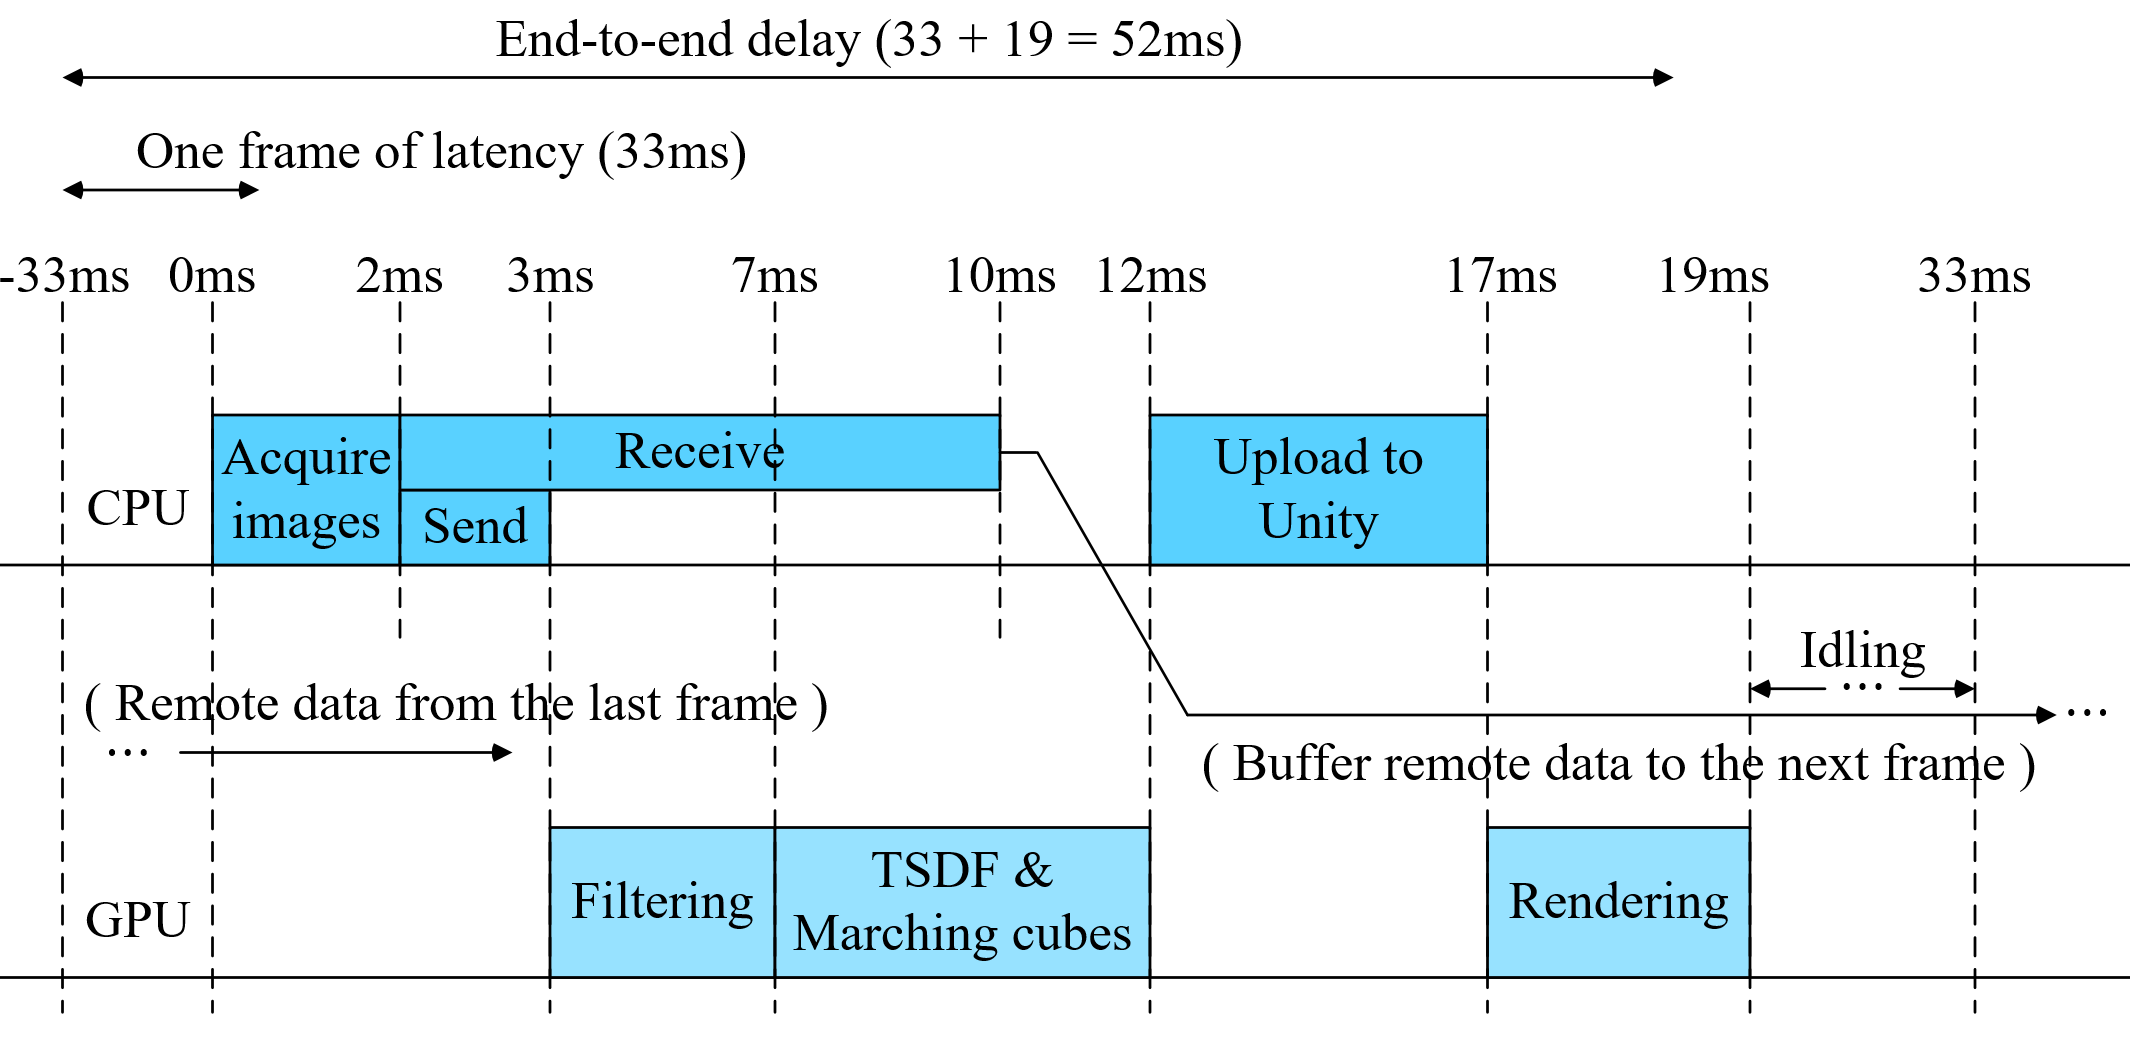
\includegraphics[width=1.0\linewidth]{figures/figure_pipeline_new3.png}
\caption{}
\label{fig:system_delay}
\end{figure}
